\documentclass[12pt]{article}
\usepackage{amsmath}
\usepackage{mathrsfs}
\usepackage{steinmetz}
\usepackage{graphicx}
\usepackage{wrapfig}
\usepackage{booktabs}
\usepackage[letterpaper, margin=1in]{geometry}
\usepackage{fancyhdr}
\pagestyle{fancy}
\fancyhead[R]{Sinusoidal Analysis}
\fancyfoot[C]{\thepage}
\renewcommand{\headrulewidth}{1pt}
\renewcommand{\footrulewidth}{1pt}
\usepackage [autostyle, english = american]{csquotes}
\MakeOuterQuote{"}
\renewcommand{\baselinestretch}{1.0}
\newcommand{\objects}[2]{%
  \leavevmode\vbox{\hbox{#1}\nointerlineskip\hbox{#2}}%
}
\begin{document}
    \section*{The Sinusoidal Source}
    \[
        v = V_m \cos (\omega t + \phi)
    \]
    \par The sinusoidal source of either current or voltage which varies as a
    sinusoid with respect to time. The equation above is the general expression
    for the voltage of an alternating source where, $V_m$ is the amplitude
    between which the voltage is bounded. The term $\omega$ gives the radial
    frequency of the function, in radians per second, and given by the
    expression $\omega = 2\pi f$, where $f$ is the frequency. Since frequency is
    given as the inverse of the period, $f = \frac{1}{T}$, this expression can
    be given as, $\omega = \frac{2\pi}{T}$.
    \par The angle $\phi$ gives the phase angle of the function for the source
    and is responsible for the translation of the value of the function at time
    $t = 0$.
    \[
        V_{rms} = \sqrt{\frac{1}{T} \int_{t_0}^{t_0+T} V_m^2 \cos^2 (\omega t +
        \phi)\ dt}
    \]
    \par This equation is used to calculate the mean value of the voltage. This
    is done by integrating the voltage squared and multiplying by the inverse of
    the difference of the bounds. The value $V_{rms}$ is used in the calculation
    of the power generated across an alternating source, however, for this
    course it will be sufficient to know that the value under the radical will
    equal $V_m^2 / 2$, giving a value for $V_{rms}$ of,
    \[
        V_{rms} = \frac{V_m}{\sqrt{2}}
    .\]
    \section*{The Sinusoidal Response}
    \begin{figure}[h]
        \centering
        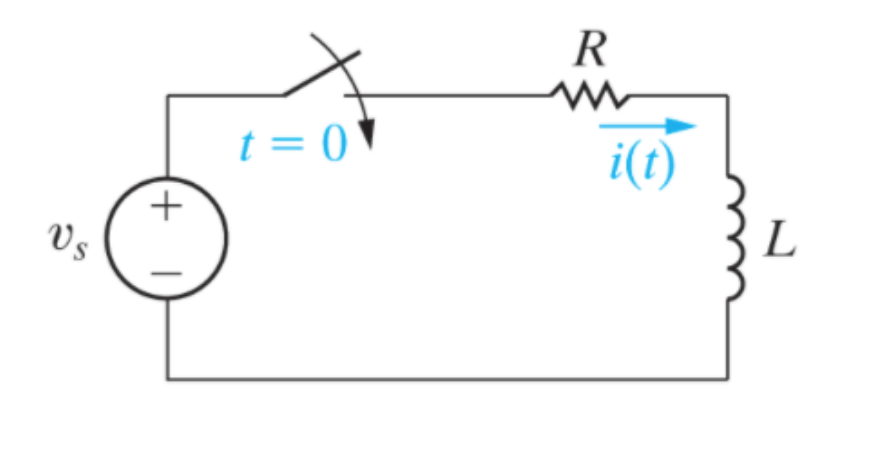
\includegraphics[width=0.45\textwidth]{Resistor-Inductor Circuit.png}
    \end{figure}
    \par For this particular circuit, the voltage at time $t=0$ will be given by
    the general for of the equation of an alternating source. Writing Kirchoff's
    Voltage Rule for this configuration we get,
    \[
        Ri + L \frac{di}{dt} = V_m \cos (\omega t\ +\ \phi)
    .\]
    \par Solving this differential equation in order to obtain the expression
    for current as a function of time, $i(t)$, we get,
    \[
        i(t) =
        \frac{-V_m}{\sqrt{R^2\ +\ \omega^2 L^2}} \cos (\phi - \theta)
        e^{-\left( \frac{R}{L} \right) t}\ +\
        \frac{V_m}{\sqrt{R^2\ +\ \omega^2 L^2}} \cos (\omega t + \phi - \theta)
    \]
    where,
    \[
        \theta = \tan^{-1} \left( \frac{\omega L}{R} \right)
    \]
    \par The first term is this expression is referred to as the homogeneous
    solution and the second, the particular solution. The difference between
    these solutions is extrapolated upon in linear differential equations.
    \section*{The Phasor}
    \[
        e^{\pm j \theta} = \cos \theta \pm j \sin \theta
    \]
    \par The Phasor is a complex number which is rooted in Euler's Identity,
    shown above and with its use, we attain a different method by which the
    cosine and sine function are defined. The cosine being the real part and the
    sine being the imaginary part of the exponential function.
    \[
        \cos \theta = \mathscr{R} \{e^{j \theta}\}
    \]
    and,
    \[
        \sin \theta = \mathscr{R} \{e^{j \theta}\}
    \]
    \par This leads to the function for the alternating voltage source to be
    written as,
    \begin{align*}
        v &= V_m \cos (\omega t + \phi) \\
          &= V_m \mathscr{R} \{e^{j (\omega t + \phi)}\} \\
          &= V_m \mathscr{R} \{e^{j \omega t} e^{j \phi}\}
    \end{align*}
    \par Since $V_m$ is a constant, it can be moved inside the argument of
    $\mathscr{R}$ without altering the expression and the equation for voltage
    becomes,
    \[
        v = \mathscr{R} \{V_m e^{j \phi} e^{j \omega t}\}
    .\]
    \subsection*{Phasor Transform}
    \[
        \textbf{V} = V_m e^{j \phi} = \mathscr{P} \{V_m \cos (\omega t + \phi)\}
    \]
    \par This is the polar form of a phasor however it can also be expressed in
    rectangular form with some manipulation.
    \[
        \textbf{V} = V_m \cos \phi\ +\ j V_m \sin \phi
    \]
    \par For the polar form it can be seen that the phasor takes the form
    $Ae^{j \phi}$, where $A$ is the amplitude and the angle can be expression
    using the angle notation, $A \phase{\phi^{\circ}}$.
    \[
        A \phase{\phi^{\circ}} \equiv A e^{j \phi}
    \]
    \subsection*{Inverse Phasor Transform}
    \[
        \mathscr{P}^{-1} \{V_m e^{j \theta}\} = \mathscr{R} \{V_m e^{j \theta}
        e^{j \omega t}\} = V_m \cos (\omega t + \theta^{\circ})
    \]
    \section*{Example 9.5 Adding Cosines Using Phasers}
    If $y_1 = 20 \cos (\omega t - 30^{\circ})$ and $y_2 = 40 \cos (\omega t +
    60^{\circ})$, express $y = y_1 + y_2$ as a single sinusoidal function.
    \[
        y = 20 \cos (\omega t - 30^{\circ}) + 40 \cos (\omega t + 60^{\circ})
    \]
    \par Using Euler's identity, the right hand side of the expression can be
    rewritten as,
    \begin{align*}
        y &= \mathscr{R} \left\{ 20 e^{-j 30^{\circ}} e^{j \omega} \right\} +
          \mathscr{R} \left\{ 40 e^{j 60^{\circ}} e^{j \omega} \right\}. \\
          &= \mathscr{R} \left\{ 20 e^{-j 30^{\circ}} e^{j \omega} + 40 e^{j
          60^{\circ}} e^{j \omega} \right\}
    \end{align*}
    \par The term $e^{j \omega}$ can be factored out and the expression becomes,
    \[
        y = \mathscr{R} \left\{ \left( 20 e^{-j 30^{\circ}} + 40 e^{j
        60^{\circ}} \right) e^{j \omega} \right\}
    \]
    \par and with that, the two phasors can be added using angle notation,
    \begin{align*}
        20 \phase{-30^{\circ}} + 40 \phase{60^{\circ}} &= (17.32 - j 10) + (20 +
        j 34.64) \\
        &= 37.32 + j 24.64 \\
        &= \boxed{44.72 \phase{33.43^{\circ}}.}
    \end{align*}
    \par With that, the sum of the two functions can be given as,
    \[
        y = \mathscr{R} \left\{ 44.72 e^{j 33.43^{\circ}} e^{j \omega} \right\}
    \]
    \par or,
    \[
        \boxed{y = 44.72 \cos (\omega t + 33.43^{\circ}).}
    \]
    \section*{Passive Circuit Elements in the Frequency Domain}
    \subsection*{The V-I Relationship for a Resistor}
    \begin{align*}
        v &= R \left[ I_m \cos (\omega t + \theta_i) \right]  \\
          &= R I_m \cos (\omega t + \theta_i), \\
          &= R I_m \phase{\theta_i}
    \end{align*}
    \par From Ohm's Law it can be deduced that current can be defined as the
    following where $I_m$ is the maximum amplitude of the current, and
    $\theta_i$ is the phase angle of the current.
    \par The phasor transform of this voltage can be written as,
    \[
        \textbf{V} = R I_m e^{j \theta_i} = R I_m \phase{\theta_i}
    .\]
    \par Since the term $I_m \phase{\theta_i}$ is the phasor representation of
    the current across the resistor, the relationship between the phasor current
    and the phasor voltage can be written simply as,
    \[
        \textbf{V} = R \textbf{I}
    .\]
    \subsection*{The V-I Relationship for an Inductor}
    \[
        v = L \frac{di}{dt} = -\omega L I_m \sin (\omega t + \theta_i)
    .\]
    \par This is the general equation for the voltage-current relationship
    across an inductor. By differentiating the phasor equation for current
    defined previously, a relationship with the voltage in phasor form can be
    determined.
    \par Replacing the sine with a cosine function,
    \[
        v = -\omega L I_m \cos (\omega t + \theta_i - 90)
    ,\]
    the phasor representation can be written as,
    \begin{align*}
        \textbf{V} &= -\omega L I_m e^{j(\theta_i - 90^{\circ})} \\
                   &= -\omega L I_m e^{j\theta_i} e^{-j 90^{\circ}}
    \end{align*}
    and since $e^{-j 90^{\circ}} = -j$,
    \begin{align*}
        \textbf{V} &= j \omega L I_m e^{j \theta_i} \\
                   &= j \omega L I_m \phase{\theta_i}
    \end{align*}
    \par Once again, the term $I_m \phase{\theta_i}$ defines the phasor
    expression for current therefore, the expression for the voltage across an
    inductor of an alternating source can be written as,
    \[
        \textbf{V} = j \omega L \textbf{I}
    .\]
    \subsection*{The V-I Relationship for a Capacitor}
    \[
        v = \frac{1}{C} \int i(t) dt = \frac{1}{C} \int I_m \cos (\omega t +
        \theta_i)\ dt = \frac{1}{\omega C}\ I_m \sin (\omega t + \theta_i)
    \]
    \par Here once again, the sine function can be converted into a cosine,
    \[
        v = \frac{I_m}{\omega C} \cos (\omega t + \theta_i - 90^{\circ})
    ,\]
    and again, writing this as an exponential,
    \begin{align*}
        \textbf{V} &= \frac{1}{\omega C}\ I_m e^{j (\theta_i - 90^{\circ})} \\
                   &= \frac{1}{\omega C}\ I_m e^{j \theta_i} e^{-j 90^{\circ}}
    \end{align*}
    and once again, since $e^{-j 90^{\circ}} = -j$,
    \begin{align*}
        \textbf{V} &= \frac{-j}{\omega C}\ I_m \phase{\theta_i}.
    \end{align*}
    \par Now, since $I_m \phase{\theta_i}$ defines the phasor $\textbf{I}$ it
    can be substituted in but also, to clean up the expression, we can bring the
    $j$ to the denominator. Since the complex number is a radical, we can in a
    sense, "reverse-rationalize" it and bring it to the denominator. The final
    expression for the relationship between voltage an current across a
    capacitor is given by,
    \[
        \textbf{V} = \frac{1}{j \omega C}\, \textbf{I}.
    \]
    \section*{Impedance}
    \[
        \textbf{V} = Z \textbf{I}
    \]
    \par The impedance is given by the term $Z$ in this equation and can be
    thought of as the "resistance" across a specific circuit element.
    \begin{table}[h]
        \centering
        \begin{tabular}{ccc}
            \toprule
            Circuit Element & Impedance & Reactance \\
            \midrule
            Resistor & $R$ & -- \\
            Inductor & $j \omega L$ & $\omega L$ \\
            Capacitor & $-j / \omega C$ & $-1 / \omega C$ \\
            \bottomrule
        \end{tabular}
    \end{table}
    \par By looking at this table, it can be seen that the value of $Z$ is
    determined by the expression that is multiplying the phasor $\textbf{I}$ in
    the voltage-current relationship equations. The impedance can be calculated
    using these expressions for the respective elements, and has a value given
    in Ohms $(\Omega)$.
    \section*{Kirchoff's Laws in the Frequency Domain}
    \subsection*{Voltage Law}
    \[
        \textbf{V}_1 + \textbf{V}_1 + \ldots + \textbf{V}_n = 0
    \]
    \par Around a closed loop, the voltage phasors across each of the elements
    in the loop will add to equal zero.
    \subsection*{Current Law}
    \[
        \textbf{I}_1 + \textbf{I}_1 + \ldots + \textbf{I}_n = 0
    \]
    \par At a junction, the current phasors traveling in from each of the paths
    of the junction will add to equal zero.
    \subsection*{Steady State Voltage Drop}
    Given that,
    \[
        \textbf{V} = 5.59 \phase{71.565^{\circ}}\ V
    ,\]
    in order to determine the steady state voltage across the elements in a loop
    being supplied by a sinusoidal source, the inverse phasor transform can be
    applied. \\
    If $\omega = 1000 rad / s$:
    \[
        v_{ss}(t) = \mathscr{P}^{-1} \left\{ \textbf{V} \right\} =
        \mathscr{P}^{-1} \left\{ 5.59 \phase{71.565^{\circ}}\ \right\}
    ,\]
    and since the inverse phaser transform is defined as,
    \[
        \mathscr{P}^{-1} \{V_m e^{j \theta}\} = \mathscr{R} \{V_m e^{j \theta}
        e^{j \omega t}\} = V_m \cos (\omega t + \theta^{\circ})
    ,\]
    the steady state voltage is given by,
    \[
        v_{ss}(t) = 5.59 \cos (1000t + 71.565^{\circ})\ V
    .\]
    \section*{Series-Parallel Simplifications}
    \subsection*{Series Combinations}
    \[
        Z_{eq} = Z_1 + Z_2 + \ldots + Z_n
    \]
    \subsection*{Parallel Combinations}
    \[
        Z_{eq} = \left( Z_1^{-1} + Z_2^{-1} + \ldots + Z_n^{-1} \right)^{-1}
    \]
    \subsection*{Voltage Division}
    \[
        V_j = \frac{Z_j}{Z_{eq}} V_s
    \]
    \section*{Example 9.9 Combining Impedances}
    For $i_s = 8 \cos (200,000t)\ A$ in the circuit:
    \begin{figure}[h]
        \centering
        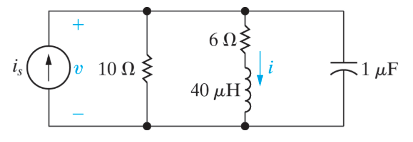
\includegraphics[width=0.65\textwidth]{Series and Parallel Impedences.png}
    \end{figure}
    \begin{enumerate}
        \item Construct the frequency-domain equivalent circuit.
        \item Find the equivalent admittance to the right of the current source.
        \item Use the equivalent admittance to find the phasor voltage
            \textbf{V}.
        \item Find the phasor current \textbf{I}, using current division.
        \item Find the steady-state expressions for $v$ and $i$.
    \end{enumerate}
    \,
    \par For the first objective, the current circuit can be transformed into
    its frequency equivalent by using the equations for the individual elements
    to determine their impedance.
    \par For the $40 \mu H$ inductor, the impedance will be equal to,
    $j(200,000)(40*10^{-6}) = j 8\ \Omega$. The same can be done for the
    capacitor, $1 / j(200,000)(1*10^{-6}) = -5j\ \Omega$. The impedance for the
    resistor is simply $R$, the resistance of the resistor, $6\ \Omega$.
    \par The current source can be written using angle notation as, $8
    \phase{0^{\circ}}$, and the final circuit will resemble,
    \begin{figure}[h]
        \centering
        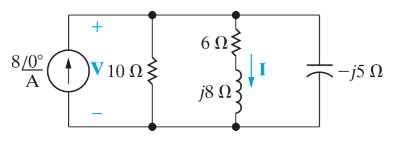
\includegraphics[width=0.6\textwidth]{Frequency-Domain Circuit.png}
    \end{figure}
    \newpage
    \par The second objective can be met by finding the admittances of the three
    branches in the circuit and then summing those values to find the equivalent
    admittance. Since admittance is defined as the inverse of impedance, for the
    right most branch, the impedance will be,
    \[
        Y_1 = \frac{1}{-j 5} = j 0.2\ S,
    \]
    for the middle branch,
    \[
        Y_2 = \frac{1}{6 + j 8} = 0.06 - j 0.08\ S,
    \]
    and the final branch, consisting of only a resistor, the admittance will be,
    \[
        Y_3 = \frac{1}{10} = 0.1\ S.
    \]
    \par Admittance is given in Seimens and in order to find the total
    admittance for the three branches, the individual values must be summed
    together,
    \begin{align*}
        Y_{eq} &= Y_1 + Y_2 + Y_3 \\
               &= 0.16 + j 0.12 \\
               &= \boxed{0.2 \phase{36.87^{\circ}}\ S.}
    \end{align*}
    \par To find the phasor voltage two characteristics of the circuit are
    required, $Z_{eq}$, the equivalent impedance, and $\textbf{I}$, the phasor
    current. Since the admittance is the inverse of the impedance, to find the
    equivalent impedance, all that needs to be done is the inverse of the
    admittance found in the previous part.
    \[
        Z_{eq} = \frac{1}{Y_{eq}} = \boxed{5 \phase{-36.87^{\circ}}\ \Omega}
    \]
    Since the current was found to be $8 \phase{0^{\circ}}$,
    \[
        \textbf{V} = (5 \phase{-36.87^{\circ}})(8 \phase{0^{\circ}}) =
        \boxed{40 \phase{-36.87^{\circ}}\ V.}
    \]
    The phasor for the branch current can be given as,
    \[
        \textbf{I} = \frac{5 \phase{-36.87^{\circ}}}{6+j 8} \left( 8
        \phase{0^{\circ}} \right) = \boxed{4 \phase{-90^{\circ}}\ A.}
    \]
    \par Using the respective phasors, the expressions for voltage and current
    as a function of time can then be written as,
    \[
        v(t) = 40 \cos (200,000t - 36.87^{\circ})\ V,
    \]
    \[
        i(t) = 4 \cos (200,000t - 90^{\circ})\ A.
    \]
\end{document}
